\section{Generative Adversarial Networks (GANs)}
\label{sec:gan_theory}

Generative Adversarial Networks (GANs) \cite{goodfellow2014generativeadversarialnetworks} are 
implicit generative models, where a neural network called the generator learns to synthesize 
realistic images by using feedback from a discriminator. The discriminator learns to distinguish 
between real and generated images, effectively critiquing the generator’s outputs, while the 
generator improves its samples based on this feedback to better fool the discriminator. Unlike 
VAEs, GANs do not explicitly maximize likelihood but instead learn to approximate the data 
distribution through adversarial training.

\subsection{Adversarial Learning Framework}

Let $\mathbf{x} \sim p_{\text{data}}(\mathbf{x})$ denote real samples from the data distribution, and let $\mathbf{z} \sim p(\mathbf{z})$ denote latent noise sampled from a simple prior (typically $\mathcal{N}(0, I)$).

The generator $G_\theta$ maps latent variables to image space:

\begin{equation}
\tilde{\mathbf{x}} = G_\theta(\mathbf{z})
\end{equation}

The discriminator $D_\phi$ outputs the probability that an input is real:

\begin{equation}
D_\phi(\mathbf{x}) \in [0,1]
\end{equation}

\subsection{Minimax Objective}

GAN training is formulated as a minimax optimization problem:

\begin{align}
\min_\theta \max_\phi \; V(D_\phi, G_\theta)
&=
\mathbb{E}_{\mathbf{x} \sim p_{\text{data}}}
\left[
\log D_\phi(\mathbf{x})
\right]
\\
&\quad +
\mathbb{E}_{\mathbf{z} \sim p(\mathbf{z})}
\left[
\log \left(1 - D_\phi(G_\theta(\mathbf{z}))\right)
\right]
\end{align}

The discriminator aims to maximize this objective, while the generator aims to minimize it.

\begin{figure}[h]
    \centering
    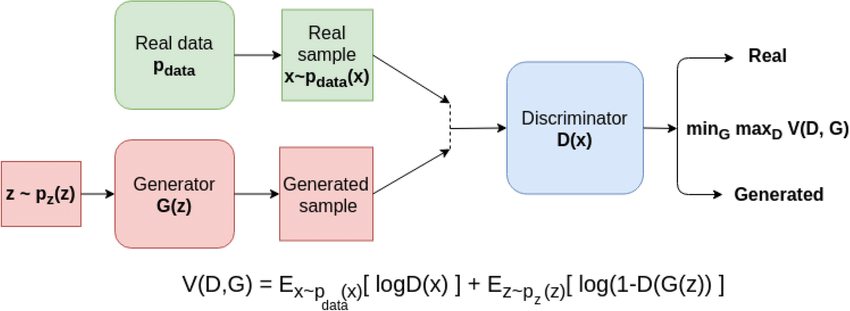
\includegraphics[width=0.8\textwidth]{model_architectures/GAN-and-loss}
    \caption{Schematic diagram of the standard GAN framework and associated loss functions. The generator $G$ learns to map random noise $\mathbf{z}$ to the data space, while the discriminator $D$ distinguishes between real and generated data. Adversarial training proceeds via the minimax objective described above.}
    \label{fig:gan_architecture}
\end{figure}



% \subsection{Optimal Discriminator}

% For a fixed generator, the optimal discriminator is:

% \begin{equation}
% D^*(\mathbf{x}) =
% \frac{p_{\text{data}}(\mathbf{x})}
% {p_{\text{data}}(\mathbf{x}) + p_G(\mathbf{x})}
% \end{equation}

% where $p_G$ is the model distribution induced by $G_\theta$.

% Substituting $D^*$ into the value function yields:

% \begin{equation}
% V(D^*, G) =
% - \log 4 +
% 2 \cdot D_{JS}\left(
% p_{\text{data}} \,\|\, p_G
% \right)
% \end{equation}

% Thus, minimizing the GAN objective corresponds to minimizing the Jensen–Shannon divergence between real and generated distributions.

\subsection{Non-Saturating Generator Loss}

In practice, the generator is trained using the non-saturating loss for stronger gradients:

\begin{equation}
\mathcal{L}_G =
- \mathbb{E}_{\mathbf{z} \sim p(\mathbf{z})}
\left[
\log D_\phi(G_\theta(\mathbf{z}))
\right]
\end{equation}

while the discriminator optimizes:

\begin{equation}
\mathcal{L}_D =
- \mathbb{E}_{\mathbf{x} \sim p_{\text{data}}}
\left[
\log D_\phi(\mathbf{x})
\right]
-
\mathbb{E}_{\mathbf{z} \sim p(\mathbf{z})}
\left[
\log \left(1 - D_\phi(G_\theta(\mathbf{z}))\right)
\right]
\end{equation}

\subsection{Wasserstein GAN}

Standard GANs may suffer from training instability due to vanishing gradients. Wasserstein GAN (WGAN) replaces JS divergence with Wasserstein distance:

\begin{equation}
W(p_{\text{data}}, p_G) =
\inf_{\gamma \in \Pi(p_{\text{data}}, p_G)}
\mathbb{E}_{(\mathbf{x},\tilde{\mathbf{x}}) \sim \gamma}
\left[
\|\mathbf{x} - \tilde{\mathbf{x}}\|
\right]
\end{equation}

Using Kantorovich–Rubinstein duality:

\begin{equation}
W(p_{\text{data}}, p_G) =
\sup_{\|D\|_L \le 1}
\mathbb{E}_{\mathbf{x} \sim p_{\text{data}}}
[D(\mathbf{x})]
-
\mathbb{E}_{\mathbf{z} \sim p(\mathbf{z})}
[D(G(\mathbf{z}))]
\end{equation}

This leads to improved training stability.

\subsection{Conditional GANs}

To control generation, GANs can be conditioned on labels $y$:

\begin{equation}
G_\theta(\mathbf{z}, y), \quad
D_\phi(\mathbf{x}, y)
\end{equation}

The objective becomes:

\begin{align}
\min_G \max_D
\;
\mathbb{E}_{\mathbf{x},y \sim p_{\text{data}}}
[\log D(\mathbf{x}, y)]
+
\mathbb{E}_{\mathbf{z} \sim p(\mathbf{z}), y}
[\log(1 - D(G(\mathbf{z}, y), y))]
\end{align}

Conditional GANs are particularly relevant in medical imaging for pathology-controlled image generation.

% \subsection{Comparison with Likelihood-Based Models}

Unlike VAEs, GANs do not require explicit likelihood modeling, no pixel-wise reconstruction term is used and generated images are typically sharper.
However, GANs exhibit  training instability, mode collapse (limited diversity) and lacks explicit latent density estimation.

% \subsection{Relevance to Medical Image Generation}

% For chest X-ray generation:

% \begin{itemize}
%     \item GANs can produce high-fidelity synthetic radiographs.
%     \item Conditional GANs allow pathology-specific generation.
%     \item However, ensuring anatomical consistency and diversity remains challenging.
% \end{itemize}
\section{DC GAN Experiments}
\subsection{Progressive GAN}

Images generated using Progressive GAN 

\begin{figure}[ht]
    \centering
    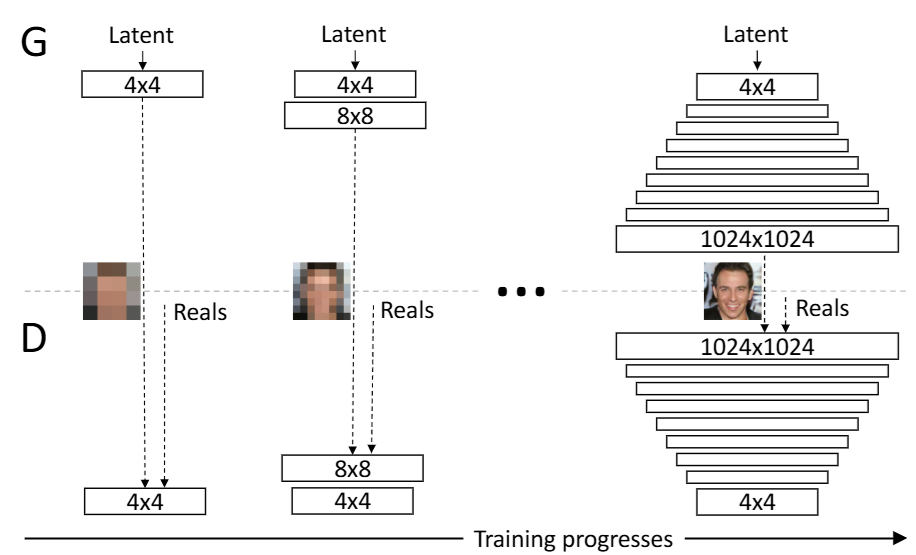
\includegraphics[width=0.85\textwidth]{model_architectures/progressive-gan.png}
    \caption{Progressive GAN architecture. Progressive growing enables synthesis of high-resolution images by starting at low resolution and incrementally adding layers to both generator and discriminator.}
    \label{fig:pro-gan-architecture}
\end{figure}



\section{Style-Based Generative Adversarial Networks}
\label{sec:stylegan_theory}

StyleGAN introduces a style-based generator architecture that improves controllability, disentanglement, and image fidelity. Unlike classical GANs that feed the latent vector directly into the generator, StyleGAN modifies the internal normalization and feature modulation process.

\subsection{StyleGAN (StyleGAN1)}

\subsubsection{Mapping Network}

Instead of directly using $\mathbf{z} \sim \mathcal{N}(0,I)$, StyleGAN first transforms it via a mapping network:

\begin{equation}
\mathbf{w} = f_{\text{map}}(\mathbf{z})
\end{equation}

where $f_{\text{map}}$ is typically an 8-layer MLP.

This transforms the latent space $\mathcal{Z}$ into an intermediate latent space $\mathcal{W}$ that is empirically more disentangled.

\subsubsection{Adaptive Instance Normalization (AdaIN)}

Each convolutional layer receives style parameters derived from $\mathbf{w}$. Let $\mathbf{h}$ denote intermediate feature maps. AdaIN is defined as:

\begin{equation}
\text{AdaIN}(\mathbf{h}, \mathbf{w}) =
\gamma(\mathbf{w})
\frac{\mathbf{h} - \mu(\mathbf{h})}{\sigma(\mathbf{h})}
+ \beta(\mathbf{w})
\end{equation}

where:
\begin{itemize}
    \item $\mu(\mathbf{h}), \sigma(\mathbf{h})$ are per-channel statistics,
    \item $\gamma(\mathbf{w}), \beta(\mathbf{w})$ are learned affine transforms.
\end{itemize}

This allows different layers to control different visual attributes (coarse-to-fine structure).

\subsubsection{Noise Injection}

Spatially uncorrelated Gaussian noise is injected into each layer:

\begin{equation}
\mathbf{h}' = \mathbf{h} + \alpha \mathbf{n}
\end{equation}

where $\mathbf{n} \sim \mathcal{N}(0,1)$ and $\alpha$ is learned per channel. This models stochastic details such as texture.

\subsubsection{Progressive Growing}

StyleGAN1 inherits progressive growing from ProGAN, gradually increasing resolution during training to stabilize convergence.

\bigskip

\subsection{StyleGAN2}

StyleGAN2 addresses artifacts introduced by AdaIN and progressive growing.

\subsubsection{Weight Demodulation}

Instead of AdaIN, StyleGAN2 incorporates style modulation directly into convolution weights.

Let convolution weights be $W$. Modulation is applied as:

\begin{equation}
W'_{i,j} = s_i W_{i,j}
\end{equation}

where $s_i$ is derived from $\mathbf{w}$.

To prevent signal amplification, weights are demodulated:

\begin{equation}
\hat{W}_{i,j} =
\frac{W'_{i,j}}
{\sqrt{\sum_k (W'_{i,k})^2 + \epsilon}}
\end{equation}

This eliminates normalization-induced artifacts and improves image fidelity.

\subsubsection{Removal of Progressive Growing}

StyleGAN2 removes progressive growing and instead uses skip connections and residual architectures, leading to:

\begin{itemize}
    \item Improved training stability
    \item Better frequency consistency
    \item Reduced texture artifacts
\end{itemize}

\subsubsection{Path Length Regularization}

To encourage smooth latent interpolation, StyleGAN2 introduces path length regularization:

\begin{equation}
\mathcal{L}_{\text{pl}} =
\mathbb{E}_{\mathbf{z}, \mathbf{y}}
\left[
\left(
\|\nabla_{\mathbf{w}} G(\mathbf{w}) \mathbf{y}\|_2 - a
\right)^2
\right]
\end{equation}

where $\mathbf{y}$ is random noise and $a$ is a running average.

This regularization encourages consistent perceptual change per unit step in latent space.

\bigskip

\subsection{StyleGAN3}

StyleGAN3 addresses aliasing artifacts and improves translation equivariance.

\subsubsection{Aliasing Problem}

Earlier StyleGAN versions produce features tied to absolute pixel coordinates. This results in:

\begin{itemize}
    \item Texture "sticking"
    \item Inconsistent translation behavior
\end{itemize}

\subsubsection{Continuous Signal Interpretation}

StyleGAN3 interprets feature maps as continuous signals sampled on a grid.

Convolution is reformulated as:

\begin{equation}
\mathbf{h}(x) =
\int
\mathbf{k}(x - \tau)
\mathbf{f}(\tau)
d\tau
\end{equation}

followed by careful low-pass filtering before resampling.

This ensures that transformations like translation correspond to phase shifts in continuous space rather than aliasing artifacts.

\subsubsection{Improved Equivariance}

StyleGAN3 enforces approximate equivariance:

\begin{equation}
G(T(\mathbf{z})) \approx T(G(\mathbf{z}))
\end{equation}

where $T$ denotes spatial transformations.

This leads to:

\begin{itemize}
    \item Reduced texture sticking
    \item Improved geometric consistency
    \item Better motion consistency in video synthesis
\end{itemize}

\bigskip

\subsection{Comparison Across Versions}

\begin{center}
\begin{tabular}{lccc}
\hline
Feature & StyleGAN1 & StyleGAN2 & StyleGAN3 \\
\hline
Mapping Network & \checkmark & \checkmark & \checkmark \\
AdaIN & \checkmark & -- & -- \\
Weight Demodulation & -- & \checkmark & \checkmark \\
Progressive Growing & \checkmark & -- & -- \\
Anti-Aliasing Design & -- & -- & \checkmark \\
Equivariance Improvements & -- & Partial & \checkmark \\
\hline
\end{tabular}
\end{center}

\subsection{Relevance to Medical Image Generation}

In medical imaging (e.g., chest X-rays):

\begin{itemize}
    \item StyleGAN1 provides controllable latent structure.
    \item StyleGAN2 improves high-frequency anatomical realism.
    \item StyleGAN3 enhances geometric consistency, reducing artificial texture artifacts.
\end{itemize}

However, GAN-based models remain limited in:

\begin{itemize}
    \item Modeling rare pathologies (mode collapse risk),
    \item Providing likelihood estimates,
    \item Ensuring full coverage of anatomical variability.
\end{itemize}

Compared to VAEs, GANs typically yield sharper images but may suffer from reduced coverage of rare pathologies due to mode collapse.